\documentclass{standalone}
\usepackage{tikz}
\usepackage[charter]{mathdesign}
\usepackage{amsmath}

\begin{document}

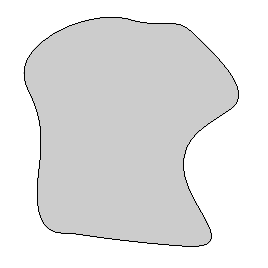
\includegraphics[width=\textwidth]{arbitraryCavity.pdf}
\begin{tikzpicture}[remember picture, overlay,shift={(-0.5\textwidth,0.5\textwidth)}]
\tikzstyle{every node}=[font=\huge]
  \foreach \x in {1,2,3,6} \draw[very thick,gray] (0,0) circle (\x);
  \foreach \x in {1,2,5} \draw[blue!50!white,very thick,dashed] (0,0) circle (0.5+\x);
  
  \draw[thick,->] (0,0) -- (1,0) node [near end,below] {$r_0$};
  \foreach \x in {1,2} \draw [->,thick] (0,0) -- (\x*10:0.5+\x) node [very near end, below right] {$r_\x$};
  \draw[thick,->] (0,0) -- (5*10:5) node [very near end, below right] {$r_N$};
  \draw[thick,->] (0,0) -- (6*10:6) node [fill opacity=0.8, fill=white,very near end,right] {$r_{N+1}=R_0$};
  \draw[very thick,dotted] (-2.5,2.5) -- (-3.5,3.5);
  
  \node at (-0.5,0) {$n_\text{in}$};
  \node[gray] at (0,-0.7) {$j=0$};
  \node[blue!70!white] at (0,-1.3) {$j=1$};
  \node[blue!70!white] at (0,-2.3) {$j=2$};
  \node[blue!70!white] at (0,-5.3) {$j=N$};
  \node[gray] at (0,-5.8) {$j=N+1$};
\end{tikzpicture}
\end{document}
